\chapter{A toy example: Learning the log linearity constant of a spatial DPP}

We will apply the MLE and the Bayesian estimation for one log linear model in a controlled environment, i.e. where the data is generated by ourselves. We will see how the Bayesian approach allows to encode more information and how the regulariser or prior affects the estimation and will quickly discuss how this impacts the noise sensitivity of the estimation.

We continue the example of the DPP on a two dimensional grid in the unit square from the first chapter. For this we note that for a \(100\times100\) grid the evaluation of the elementary probabilities 
\[ f_{\mathbf Y|\Theta}(A|\theta) = \frac{\det(L(\theta)_A)}{\det(L(\theta) + I)} \]
would involve the calculation of a determinant of a \(10^4\times 10^4\) matrix and even the storage of such a matrix would pose a problem since it consists of \(10^8\) numbers. If the storage of a real number is done in the double-precision floating-point format, it takes \(64\si{bit}\) per number and the space required to store the entire matrix is \(64\times 10^8\si{bit} = 800\si{MB}\), so almost one Gigabyte.\footnote{One byte is defined to be \(8\) bits. The units of Megabytes and Gigabytes are defined in the familiar way and denoted by \(\si{MB}\) and \(\si{GB}\) respectively.} This makes even the computation of the log likelihood function very time consuming, let alone its maximisation. Because of those computational hindrances we will decrease the size but the ideas remain exactly the same.

\begin{emp}[Setting]
We set
\[\mathcal Y \coloneqq 39^{-1} \left\{ 0, \dots, 39\right\}^2 \]
and obtain a \(40\times 40\) grid in the unit square. We again choose \(\mathcal R \coloneqq \mathcal Y \) and \(f\) to be
\[f(x) \coloneqq \exp\left( - 8\cdot x^2\right) \]
and set
\[(\phi_i)_j\propto f(\left\lVert i - j \right\rVert) \quad \text{for } i, j\in\mathcal Y.\]
Further we choose the qualities to be be decreasing with the distance from the centre \(m\) of the and set
\[q_i\coloneqq e^6 \cdot \exp\big(-10 \left\lVert i - m \right\rVert\big) = \exp\big( - 10\left\lVert i - m \right\rVert + 6\big). \]
\end{emp}

The goal is to estimate the two parameters that characterise the qualities, which are \(e^6\) and \(-10\). In order to do this we note that the qualities are given by a log linear model since we have
\[q_i = \exp(\theta_0^Tf_i) \quad \text{where } f_i = \begin{pmatrix}
\left\lVert i - m \right\rVert \\ 1
\end{pmatrix} \text{ and } \theta_0 = \begin{pmatrix}
-10 \\ 6
\end{pmatrix}.\]

Hence we should be able to estimate this log linearity constant \(\theta\in\mathbb R^2\) based on some data that is distributed according to this DPP. To do this we generate \(n=20\) samples \(Y_1, \dots, Y_n\) from the DPP using the sampling algorithm introduced in the first chapter.

\section{MLE and regularised MLE}

In order to perform the maximum likelihood estimation for the log linearity constant, we need to fix a similarity kernel \(\hat S\), but since we know the exact kernel, we can simply set \(\hat S_{ij} \coloneqq \phi_i^T\phi_j\). Then we maximise the log likelihood over \(\mathbb R^2\) using a pre-implemented optimisation algorithm in R. The resulting estimate was
\begin{equation}\label{mletheta}
\hat\theta = \begin{pmatrix}
-10.000250 \\ 6.007382
\end{pmatrix}
\end{equation}
but from the consistency results we already knew that it should be close to the actual parameter for large sample sizes. Since we also want to investigate the effect of a regulariser, we define two different regularisers
\[R_1(\theta)\coloneqq -\frac{\left\lVert \theta \right\rVert^2}{2^4} \quad \text{and } R_1(\theta)\coloneqq -\frac{\left\lVert \theta \right\rVert^2}{2} \]
as a regulariser. Note that those corresponds to the priors
\begin{equation}\label{toyprior}
f_{\Theta_1}(\theta) = \exp\left(-\frac{\left\lVert \theta \right\rVert^2}{2^4}\right) \quad \text{and } f_{\Theta_2}(\theta) = \exp\left(-\frac{\left\lVert \theta \right\rVert^2}{2}\right)
\end{equation}
which are -- up to scaling -- Gaussian priors with different variance. Under those regularisations, the respective MAP estimators obtained were
\[\hat\theta_1 = \begin{pmatrix}
-9.870850 \\ 5.952101
\end{pmatrix} \quad \text{and } \hat\theta_1 = \begin{pmatrix}
-9.050763 \\ 5.597739
\end{pmatrix}.\]
It is not surprising that regularised MLEs are closer to zero, since the regulariser is built to penalise large parameter values. Further the effect of the Gaussian prior with smaller variance -- which is the second one -- is larger, which is consistent with the heuristic explanation that it cooperates a stronger prior believe, since it expects the parameter to be close to zero.

We chose the sample size of \(n=20\) relatively small and want to show the effect the sample size has on the estimation. Obviously, we know from the second chapter that the different MLE will converge to the actual parameter. To show this convergence in our case, we iteratively raised the sample size from \(1\) to \(30\) and obtained the maximum likelihood estimators that are shown in Figure \ref{fig:learningcurve}. We can see that a stronger regularisation leads to a slower convergence, which is to be expected since it takes longer for the contribution \(\frac1n \cdot R\) to the maximised function to decrease.
\begin{figure}[h!]
	\centering
	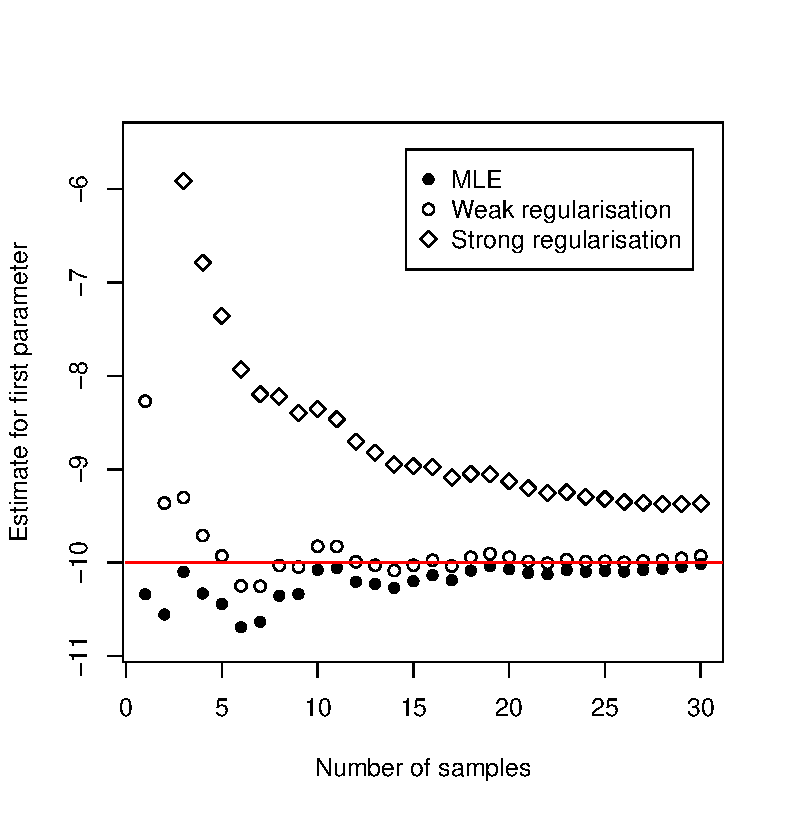
\includegraphics[width=0.49\textwidth]{figures/Learning-curve-comparison-first-parameter-final}
	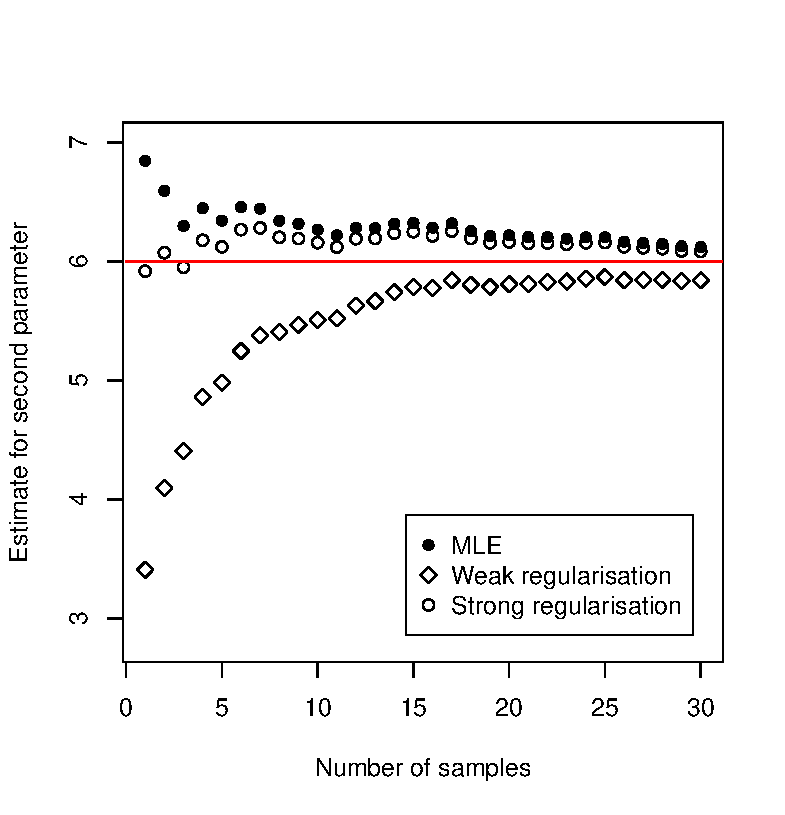
\includegraphics[width=0.49\textwidth]{figures/Learning-curve-comparison-second-parameter-final}
	\caption{Plot of the progression of the MLE and regularised MLE. The real parameter is marked by the red lines and with increased sample size they both estimators are within a reasonably small margin.}
	\label{fig:learningcurve}
\end{figure}

In the light of the comparison of the different regularisers to the unregularised MLE and also the true parameter values, it is evident that the first regularisation \(R_1\) is more suitable. We will also explain how one can compare those two regularisers without knowing the true parameter values or even without solving the maximisation problem assiciated with the MAP estimation.

\section{Bayesian estimation using MCMC methods}

We will use the same data set consisting of \(n=20\) samples and will use the first prior in \eqref{toyprior} since we have seen that it is more appropriate and will see that also the Bayes factor strongly supports this choice. The posterior of the log linearity parameter is given by
\[f_{\Theta|\mathbf Y^n}(\theta|Y_1, \dots, Y_n) \propto f_\Theta(\theta) \prod_{i=1}^n \frac{\det(L(\theta)_{Y_i})}{\det(L(\theta) + I)}.\]
and we will use the MH random walk to approximate it. But before we do this, we will shortly discuss how the Bayes factor can be used to decide between two different priors if one has not access to the unregularised and regularised MLE like we did before.

\subsubsection{Comparing the different priors via the Bayes factor}

We have introduced the Bayes factor as the ratio of the total observation probabilities under two models. In order to compare the two different priors \eqref{toyprior}, we need to integrate the observation probabilities over the parameter space, i.e. compute the integrals
\[ \int_{\Theta} f_{\mathbf Y^n| \Theta}(Y_1, \dots, Y_n| \theta)f_{\Theta_i}(\theta)\nu(\mathrm{d}\theta) \]
which we will do numerically. The order of magnitude of the approximated Bayes factor between the two models arising from the priors \eqref{toyprior} was \(10^{22}\) which strongly supports the claim that the first prior is the more sensible choice. Therefore we will only work with this one in the remainder.

It shall be noted that the numerical integration carried out above can only be performed in an efficient way if the parameter space \(\Theta\) is rather low dimensional. If this is not the case one can exploit probabilistic approaches based Monte Carlo simulations to calculate this normalisation constant. Details on such approaches can be found in the section on Monte Carlo integration in \cite{robert2013monte}.

\subsubsection{Approximation of the posterior using MCMC simulations}

In order to approximate the posterior density through a MH random walk we proceed in the following steps.
\enlargethispage{.6cm}
\begin{emp}[First burn in to find a starting point]
In the first phase we want to find an area of high density and in order to do this we simulate MH random walks with different starting positions and try to identify the regions where they get stuck in. This will typically happen in areas of at least locally highest probability. We have already seen that in order to obtain a reasonable MH random walk one has to choose a suitable proposal family. We use Gaussian proposals \(f(\cdot| \theta)\) that are centered at \(\theta\) and adjust the variance such that we obtain an acceptance rate of roughly \(25\%-75\%\).

Although there is no rigorous method to choose the variance of the proposal distribution at this point we make to general observations. A very high acceptance rate hints to the fact that every proposed step is within a region of almost equal density and hence one probably has to increase the variance and hence the proposed step size. On the other hand if the acceptance rate is close to zero is usually due to the fact that one proposes mostly steps into areas of very low density and hence it is reasonable in most cases to decrease the variance.

Once the variance is adjusted we run a first simulation of length \(2\cdot10^2\) in order to see where the MH random walk is going to focus. We take the mean value of the second half of the samples as a measure of the area where the MH random walk spends most of its time. Here, we neglect the first half since it is very highly dependent on the starting point and it shall be noted that if a state of the Markov chain has high density, the chances are rather high that it will stay there for a few more steps and hence this point is weighted more heavily in the mean of the random walk. The positions of the Markov chain are shown in Figure \ref{fig:findingstart} for different starting positions of the MH random walk and we notice that the mean of their second half hardly depends on the initial state.

\begin{figure}[h!]
	\centering
	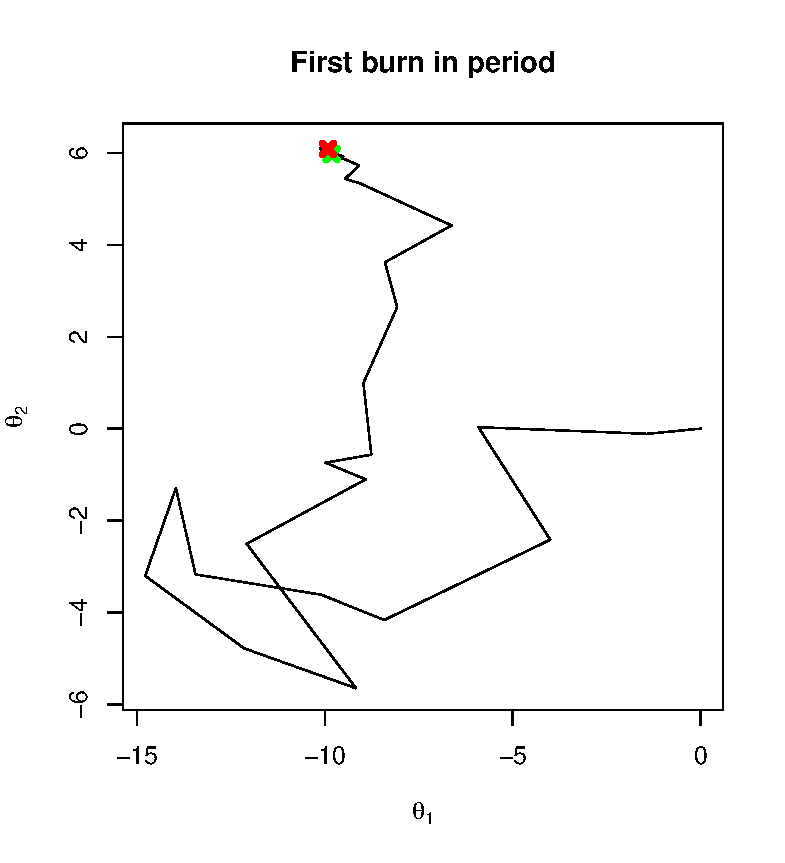
\includegraphics[width=0.49\textwidth]{figures/first-burn-in-new-2}
	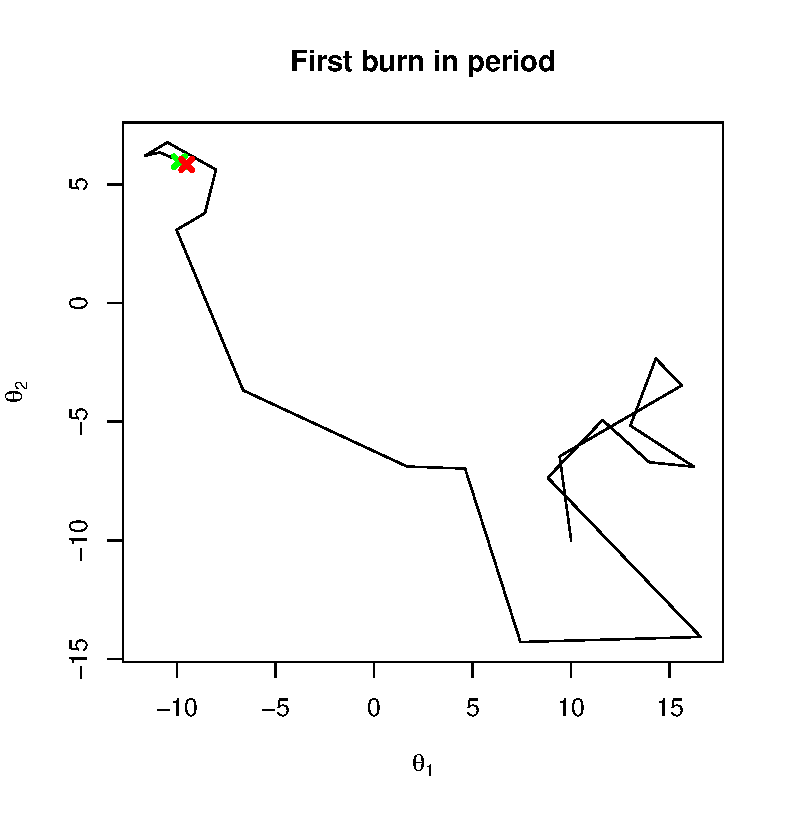
\includegraphics[width=0.49\textwidth]{figures/first-burn-in-second-start-new}
	\caption{A plot of the first burn in period with two different starting points -- the origin and \((10, -10)\). The regularised MLE for the log linearity constant is marked by the green cross and the mean of the second half of the random walk by the red cross.}
	\label{fig:findingstart}
\end{figure}

Further the plots of the states of the Markov chain in Figure \ref{fig:MCplot} show that the acceptance rate drops significantly after roughly \(20\) steps. This is a sign that we were successful in the process of finding an area with high density, since a lot of rejections imply, that the proposed points had significantly lower density. 

\begin{figure}[h!]
	\centering
	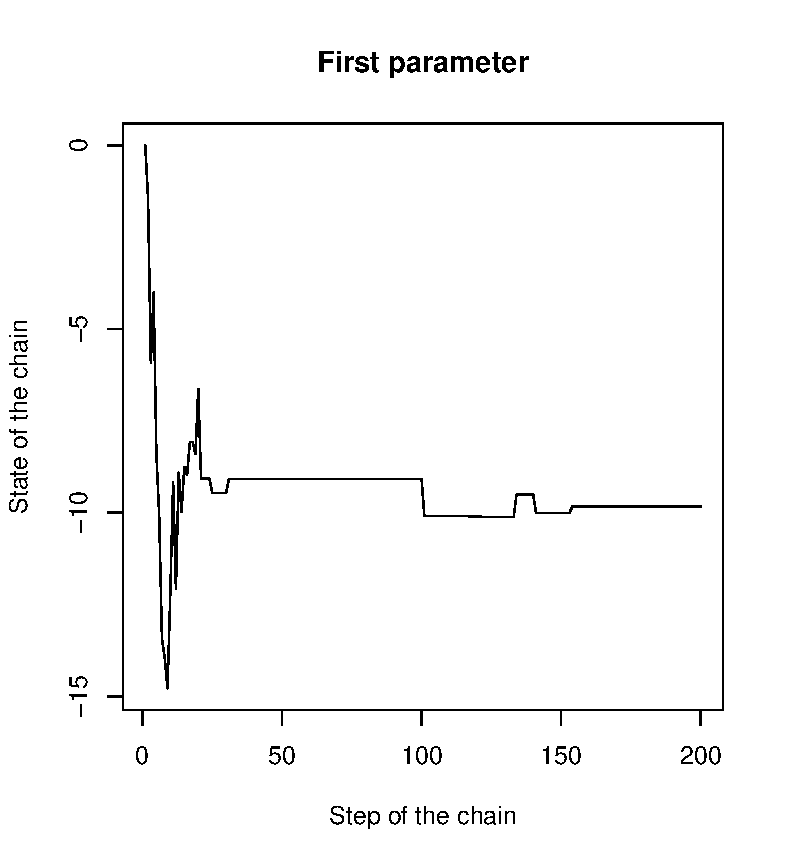
\includegraphics[width=0.49\textwidth]{figures/first-parameter-new-2}
	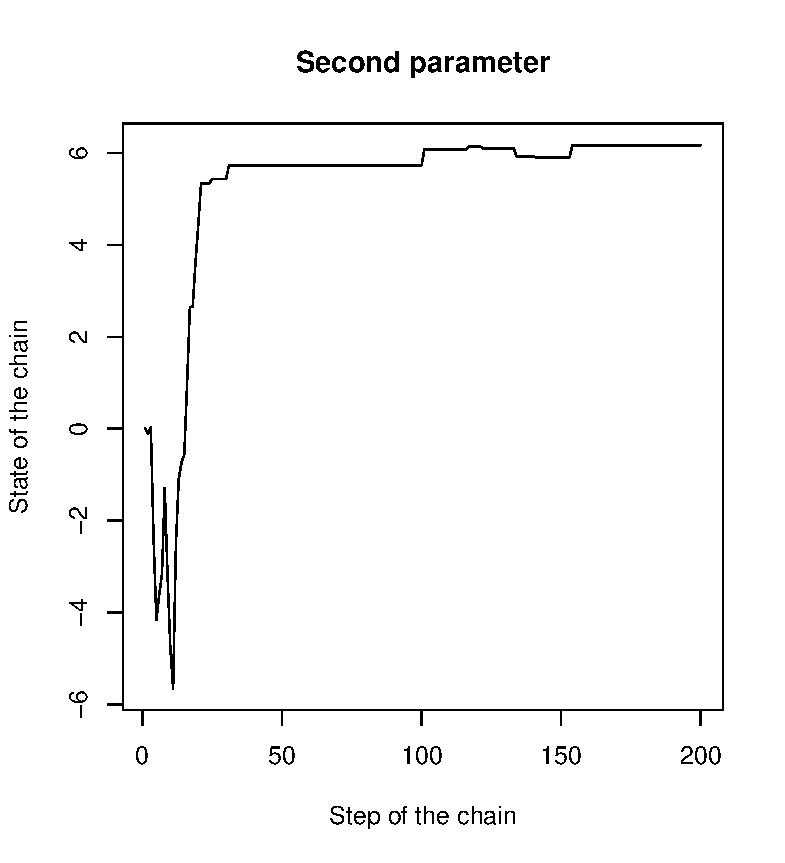
\includegraphics[width=0.49\textwidth]{figures/second-parameter-new-2}
	\caption{Plots of the two state parameters of the MH random walk starting at the origin. The acceptance rate drops significantly and hardly any proposals are accepted.}
	\label{fig:MCplot}
\end{figure}

One could argue that it would be reasonable to choose the (regularised) MLE as a starting point for the random walk. However, since we partly motivated the Bayesian approach to be an alternative to the infeasible maximum likelihood estimation for the elementary kernel \(L\), we presented the procedure above that can also be used for the estimation of \(L\).
\end{emp}

\begin{emp}[Second burn in to tune the proposal]
We use the second burn in period to tune the proposal according to \ref{tuning} for the final simulation. To do this we first select a starting point according to the result of the first burn in period. Then we adjust the variance of the Gaussian proposals such that we obtain a reasonable acceptance rate. The variance of the proposals will be much smaller than the one of the first burn in since we have seen in the state plots of the first burn in period that the acceptance rate decreased heavily. In a heuristic way it can be said that one now works �locally� and tries to explore the finer structure of the distribution and has to take smaller steps in order to do so.
We run this MH random walk for \(5\cdot10^2\) samples which are shown in Figure \ref{fig:tuning} and calculate their empirical covariance \(\Sigma\in\mathbb R^{2\times 2}\). We see that the points are located around the regularised MLE and we can get a first idea along which direction the parameter is more uncertain.


\begin{figure}
	\centering
	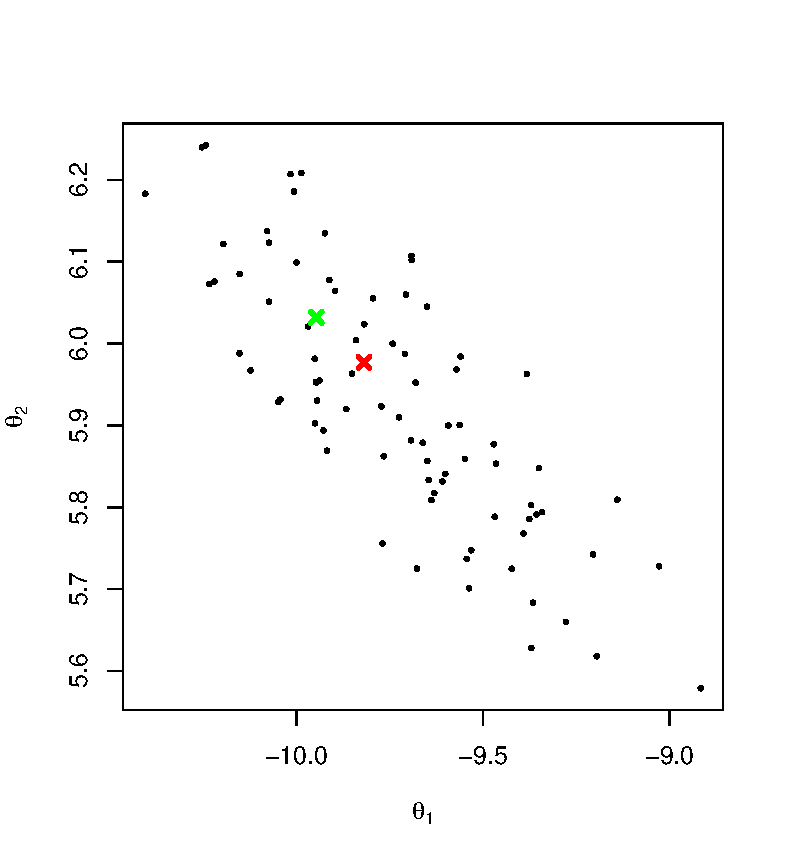
\includegraphics[width=0.56\textwidth]{figures/second-burn-in-new-2}
	\caption{A plot of the samples of the MH of the second burn in period. One can see how the points are distributed around the regularised MLE which is marked red, the MLE is marked green. Their empirical covariance will be used to tune the proposal.}
	\label{fig:tuning}
\end{figure}
\begin{figure}[h!]
	\centering
	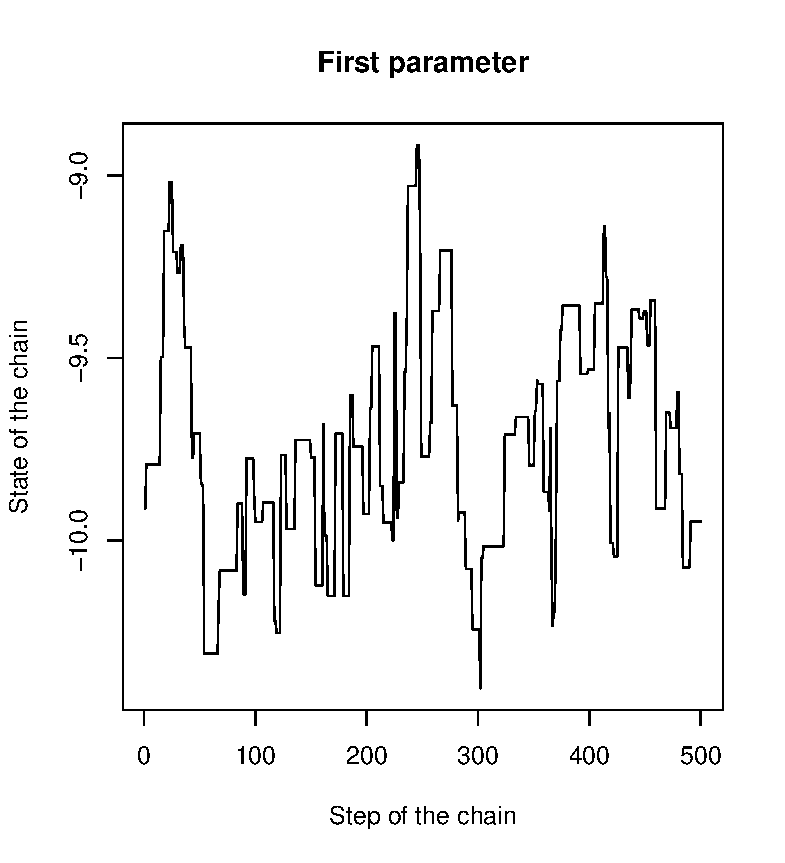
\includegraphics[width=0.49\textwidth]{figures/bayes-second-burn-in-first-parameter-new-2}
	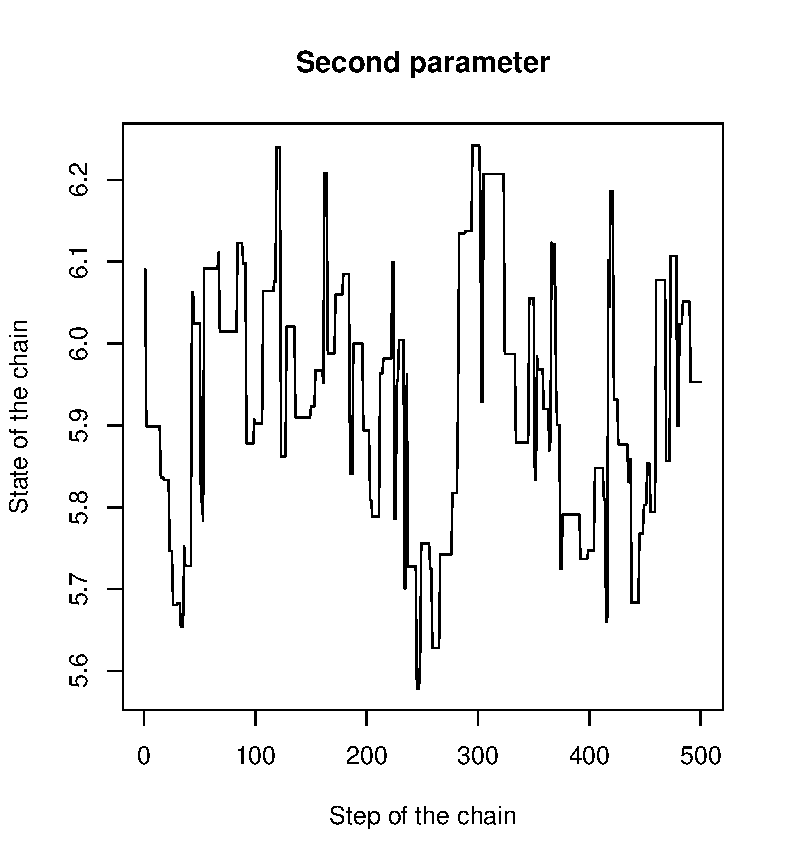
\includegraphics[width=0.49\textwidth]{figures/bayes-second-burn-in-second-parameter-new-2}
	\caption{State plots of the second burn in period. One can see that the acceptance rate does not change like in the first burn in.}
	\label{fig:mixim-tuning}
\end{figure}
\end{emp}

\enlargethispage{.3cm}
\begin{emp}[The actual MCMC simulation]
In this final step we simulate a MH random walk of length \(10^4\) and with the same starting point as in the second step. Now we use the prior adjusted according the second burn in period. This means we choose \(f(\cdot|\theta)\) to be the density of a normal distribution centered at \(\theta\) and with covariance \(\Sigma\). This leads to a higher acceptance rate of \(60\%\) compared to \(21\%\) in the second burn in period which can also be seen in the according state plots in Figure \ref{fig:mixim-tuning} and \ref{fig:mixim-tuning-final}. Further we see in Figure \ref{fig:acf-sbi-final} that the auto correlation function decreases faster with this tuned proposal.
\begin{figure}
	\centering
	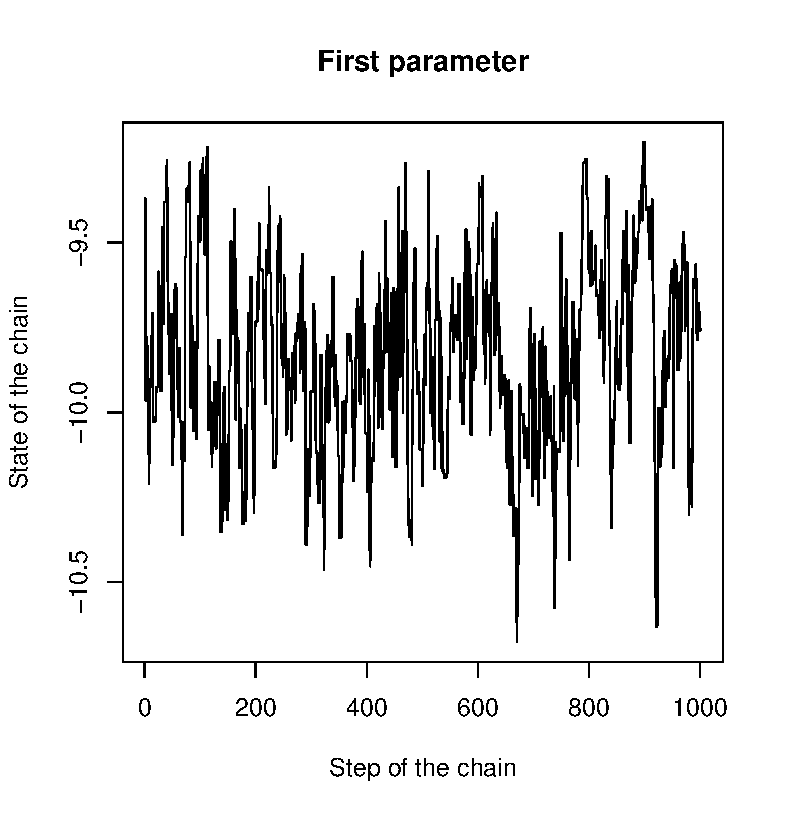
\includegraphics[width=0.49\textwidth]{figures/bayes-final-MH-first-parameter-new}
	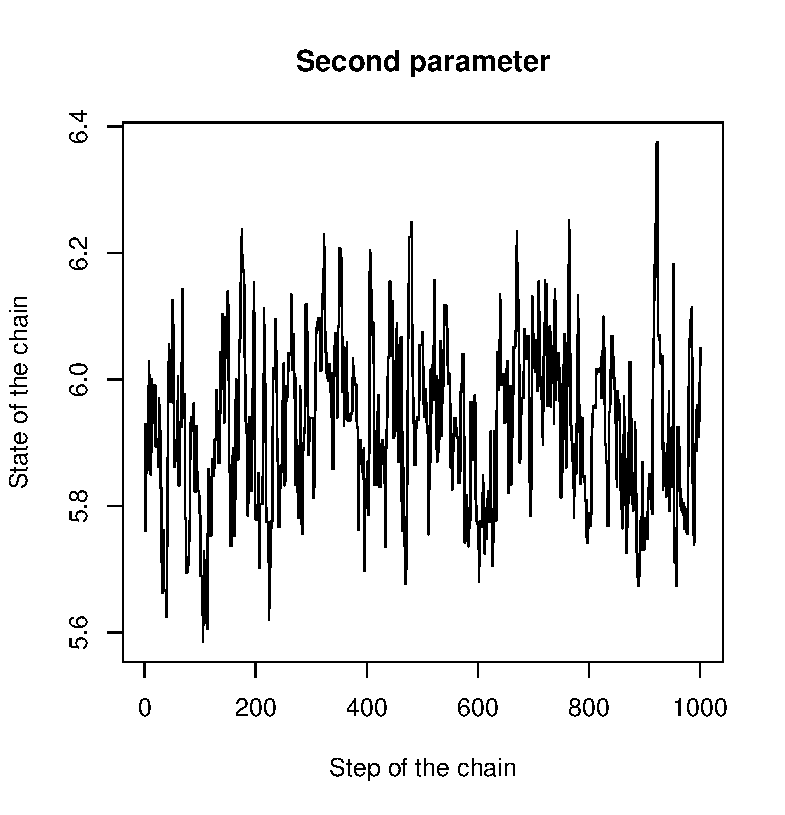
\includegraphics[width=0.49\textwidth]{figures/bayes-final-MH-second-parameter-new}
	\caption{State plots of the 	final MH random walk on the bottom. One can see how the tuned proposal gives a higher acceptance rate than in the second burn in period.}
	\label{fig:mixim-tuning-final}
\end{figure}
\begin{figure}
	\centering
	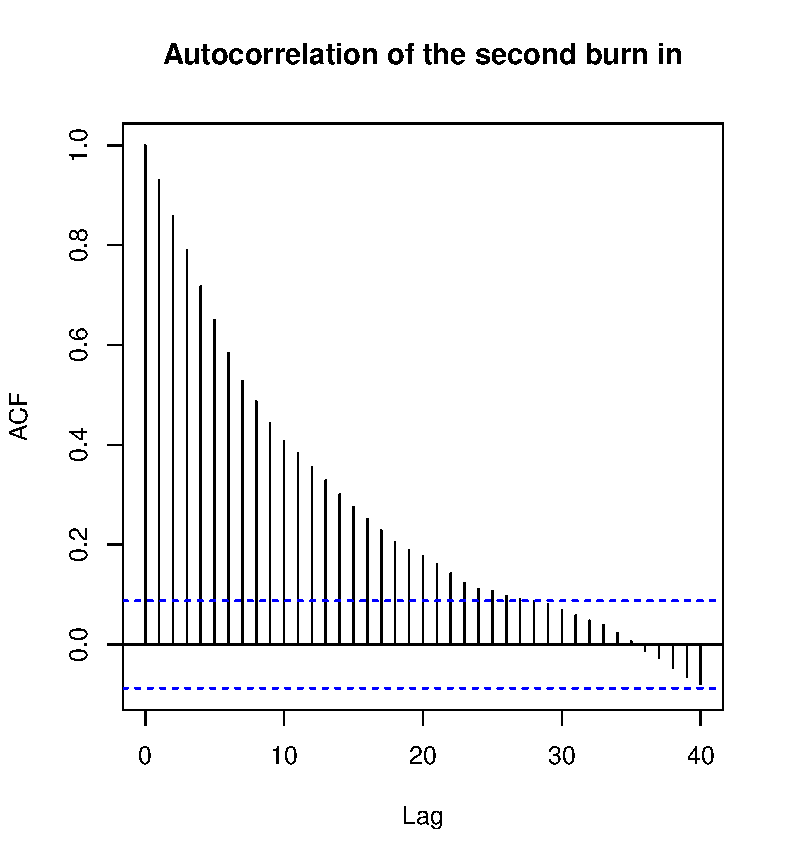
\includegraphics[width=0.46\textwidth]{figures/bayes-acf-second-burn-in-new-2}
	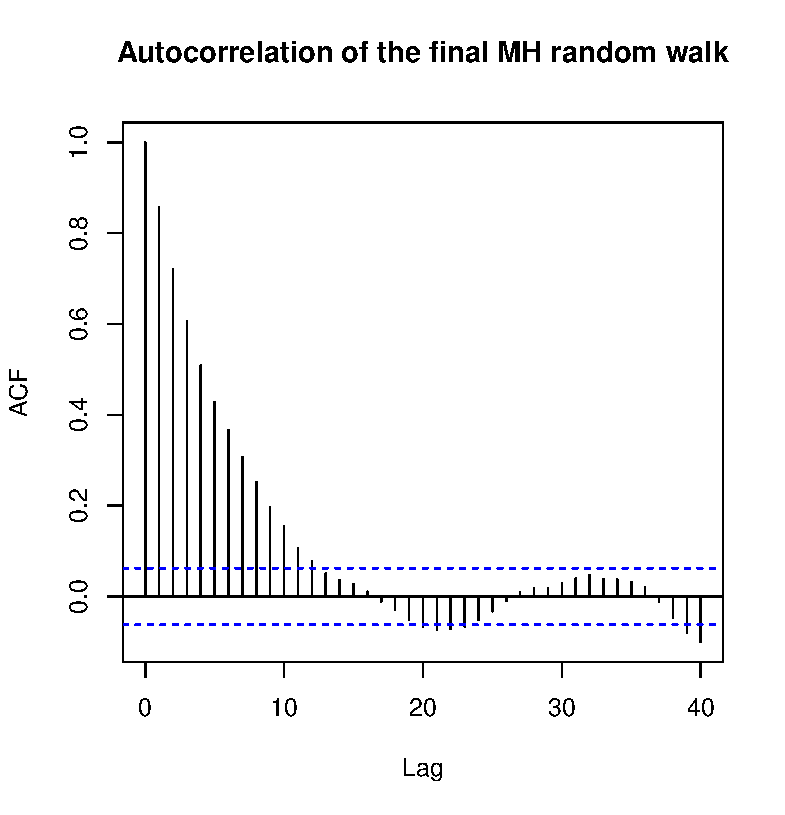
\includegraphics[width=0.49\textwidth]{figures/bayes-acf-final-MH-new}
	\caption{A plot of the autocorrelation functions of the second burn in period and the final MH random walk. The latter one decreases faster which hints to a faster convergence due to the tuned proposal distributions.}
	\label{fig:acf-sbi-final}
\end{figure}
Finally we use a pre-implemented interpolation method to obtain a smoothed twodimensional histogram -- also called a heat plot -- which is shown in Figure \ref{fig:MHrw}.
\end{emp}
\clearpage
\begin{figure}
	\centering
	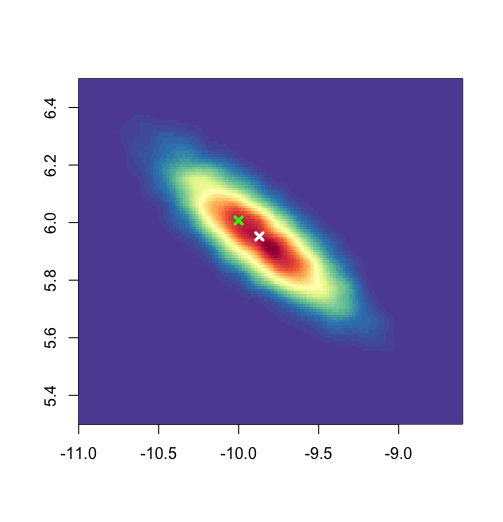
\includegraphics[width=0.55\textwidth]{figures/bayes-mle-and-regmle-new}
	\caption{Heat map of the MH random walks with \(10^4\) iterations. The regularised MLE estimator is shown as a white and the MLE as a green cross. The regularised MLE is the maximum of the (approximated) posterior.}
	\label{fig:MHrw}
\end{figure}
\begin{emp}[Gelman-Rubin diagnostic]
In order to justify the length of \(10^4\) of our final MCMC simulation for the approximation of the posterior we use the Gelman-Rubin diagnostic. Hence, we run a second chain with a random starting value sampled from a Gaussian distribution centered around the mean of the second half of the first burn in period and with twice the variance of the second burn in period. Then we use the pre-implemented R function {\tt gelman.diag} that computes the \(\hat R\) value and an upper estimate for it and obtain the following results. 
\begin{table}[h!]
\centering
\begin{tabular}{ |c|c|c| } 
 \hline
  & \(\hat R\) value & upper estimation of \(\hat R\) \\ \hline
  First parameter & 1.01 & 1.06 \\ \hline
  Second parameter & 1.02 & 1.09 \\ \hline
\end{tabular}
\caption{Table with \(\hat R\) values for both coordinates of the parameter including upper estimates.} \label{tab:R-hat}
\end{table}

The small \(\hat R\) values imply that the length of the MH random walk was not too short. On the other hand Figure \ref{fig:R-hat} shows a plot of the evolution of the \(\hat R\) value with increasing length of the chain and it suggests that the length of the chain was not unreasonably long.

\begin{figure}[h!]
	\centering
	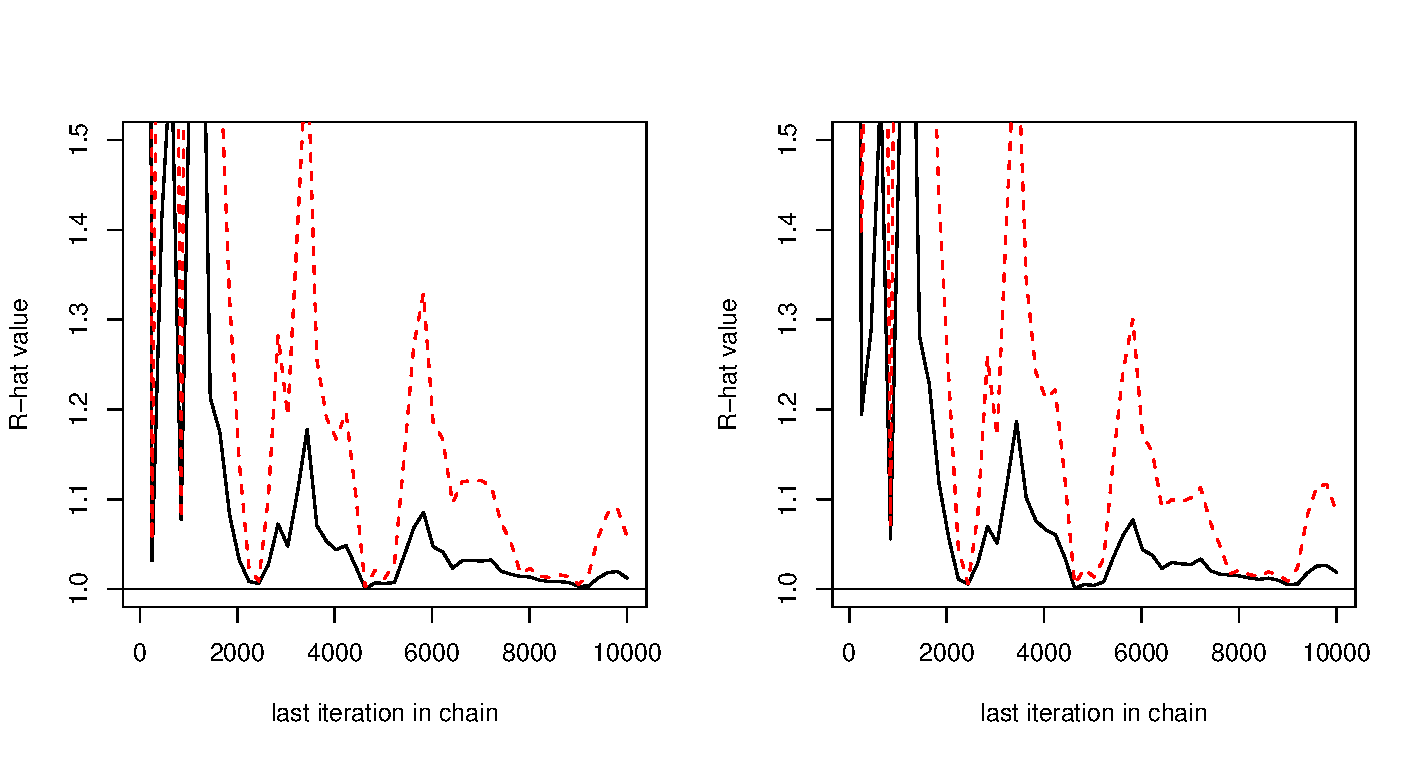
\includegraphics[width=0.9\textwidth]{figures/R-hat-final-chain}
	\caption{Plot of the evolution of the \(\hat R\) value for first (left) and second (right) coordinate of the parameter in dependency of the length of the Markov chain. The upper estimates for the \(\hat R\) value are depicted in red.}
	\label{fig:R-hat}
\end{figure}

\end{emp}

\subsubsection*{Bayesian approach without prior}

We have seen that the prior or regulariser influences the estimation and will often lead to worse estimates. However, we have discussed shortly how we can follow a generalised Bayesian approach without a prior which results in having the likelihood function as a posterior,
\[f_{\Theta|X}(\theta|x) = f_{X|\Theta}(x|\theta).\]
In order to see that the MCMC approximation still works for this function, we note that
\[\mathrm{d}\pi \coloneqq f_{\Theta|X}\cdot\mathrm{d}\mu \]
is a \(\sigma\)-finite measure on the parameter space \(\Theta\). To approximate this measure, one can use the following more general version of the ergodic theorem (cf. Theorem 17.3.2  \cite{meyn2012markov}).

\begin{theo}[Ergodic theorem]\label{ergTheo2}
Let \((X_n)_{n\in\mathbb N}\) be a Markov chain with \(\sigma\)-finite stationary distribution \(\pi\) and let 
\[\hat{\mathbb P}_n \coloneqq \frac1n \sum_{i=1}^n \delta_{X_i} \]
be the empirical measures associated with the Markov chain. Then the following two statements are equivalent:
\begin{enumerate}
\item For all \(\pi\)-integrable functions \(f, g\) with \(\int g(x)\pi(\mathrm{d} x)\ne0\) we have
\[\frac{\int f(x) \hat{\mathbb P}_n(\mathrm{d} x)}{\int g(x)\hat{\mathbb P}_n(\mathrm{d} x)} \xlongrightarrow{n\to\infty} \frac{\int f(x)\pi(\mathrm{d} x)}{\int g(x)\pi(\mathrm{d} x)}. \]
\item The Markov chain \((X_n)_{n\in\mathbb N}\) is  Harris recurrent.
\end{enumerate}
\end{theo}

This implies directly that the restrictions of \(\hat{\mathbb P}_n\) onto sets of finite measure \(\pi(A)<\infty\) converge weakly towards \(\pi\) up to normalisation. The argument for the stationarity of the \(\sigma\)-finite measure \(\pi\) stays exactly the same as before. 
\begin{figure}[h!]
	\centering
	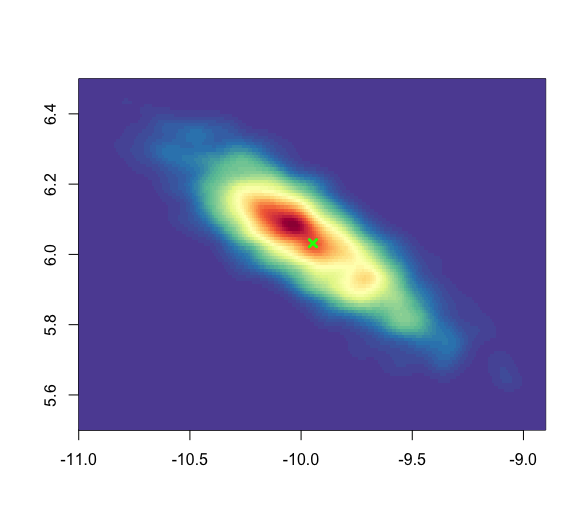
\includegraphics[width=0.6\textwidth]{figures/bayes-mle-withou-prior-new}
	\caption{Heat map of the MH random walks with \(10^4\) iterations. The regularised MLE estimator is shown as a white and the MLE as a green cross. The MLE is the maximum of the (approximated) likelihood.}
	\label{fig:MHrwwup}
\end{figure}
Hence, we can take a completely analogue approach for the approximation of the likelihood function, but we only present the result of the third and final MCMC simulation in Figure \ref{fig:MHrwwup}.

It is evident from both, theoretical considerations and the experimental results of the maximum likelihood estimations and the approximations of the posterior that the regulariser or prior always forces the estimation closer to the origin. Obviously this can make the estimation better, if for example the unregularised MLE is larger than the actual parameter, but then it makes the estimation better by pure luck. We will see later that the influence of the prior can be a little bit more positive if the data is perturbed by random noise.

\subsubsection*{A naive approximation of the posterior}
\enlargethispage{.1cm}
The motivation for the use of MCMC methods was that one wants to obtain an approximation of the posterior. We present here a different and naive approach, which works a lot faster at least in our toy example. However, we will see later that this approach suffers from what is known as the \emph{curse of dimensionality},\footnote{This name is used for pretty much all phenomena that grow exponentially with the dimension of the problem.} i.e. the time needed to perform it will grow exponentially with the dimension of the parameter that should be estimated.

Let us assume that we have performed the two burn in periods of the MH random walk presented above. Then we roughly know the location of the high density from the first burn in period and also the approximate shape of it from the second one. Now we place a \(40\times 40\) grid above this box and evaluate the unnormalised posterior at those grid points. Then we use an interpolation algorithm to obtain an approximation of the unnormalised posterior density. This interpolation usually comes in a quite simply form -- for example piecewise linear -- and can therefore by explicitely expressed and integrated in order to normalise the approximate posterior. The results for this approach can be seen in Figure \ref{fig:directHeatMaps} and we will discuss the advantages and hindrances in the next paragraph.

\begin{figure}[h!]
	\centering
	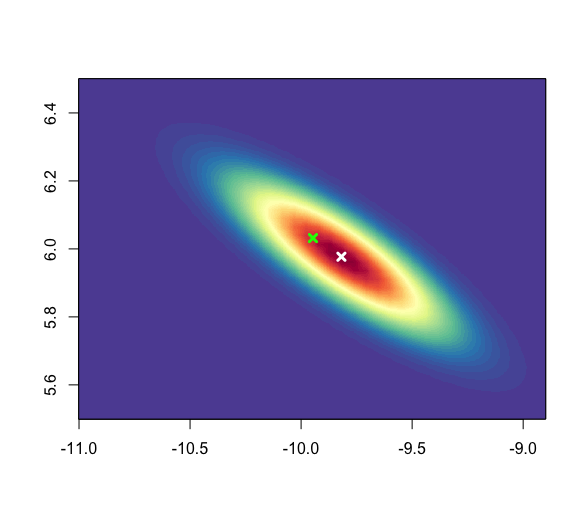
\includegraphics[width=0.49\textwidth]{figures/posterior-direct-approx-new}
	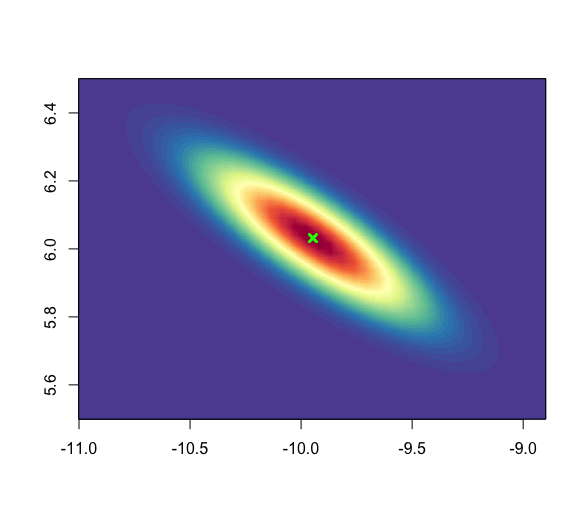
\includegraphics[width=0.49\textwidth]{figures/likelihood-direct-approx-new}
	\caption{Approximations of the posterior (left) and of the likelihood function (right) obtained by the interpolation between breakpoints. Just like in the approximations using MCMC methods, the reguralised MLE is marked white and the MLE green.}
	\label{fig:directHeatMaps}
\end{figure}

\subsubsection*{Complexity of the different approaches}

In large examples the evaluation of the likelihood function
\[f_{\mathbf Y^n|\Theta}(Y_1, \dots, Y_n|\theta) \propto \prod_{i=1}^n \frac{\det(L(\theta)_{Y_i})}{\det(L(\theta) + I)} \]
involves the computation of a \(N\times N\) matrix. This can be done explicitly using Gauss elimination which does not change the determinant -- at least up to a sign -- and can be performed in at most \(N^3\) steps, cf. \cite{valiant1979complexity}.\footnote{Actually one can even do better, but those algorithms come with greater implementation challenges.} Hence, the time needed for the computation of the likelihood function can be bounded -- up to a constant -- by
\[N^3 + \sum_{i=1}^n \left\lvert Y_i \right\rvert^3 \le (n+1) \cdot N^3\]
and we say it can be performed in \(O(N^3)\) time.\footnote{See also the Landau or �big \(O\)� notation in the nomenclature.} 
In practice this will take a significant amount of time and this was also the motivation for the variational MCMC methods. For example in our toy example the computation took roughly \(1.5\) seconds on a \(1.8\si{GHz}\) Intel Core i5 with \(8\si{GB}\) RAM\footnote{I used a MacBook Air from 2012.} using the determinant algorithm in R.

For a single step of the MH random walk the unnormalised posterior needs to be evaluated twice for the computation of the acceptance threshold \(\rho(x, y)\), cf. \eqref{threshold}. Usually one will work with a prior that is easy to compute and with a proposal that can be simulated fast and hence we will neglect its contribution and thus one step of the performance of one MH random walk can be carried out in \(O(N^3)\) time. If \(T\) denotes the length of the MCMC method, the time needed for its simulation is 
\begin{equation}\label{complexityMCMC}
O\left( T\cdot N^3\right).
\end{equation}

In the final step of the MH random walk, we set \(T=10^4\) as the length and this relates to an approximate simulation time of
\[10^4 \cdot 2\cdot 1.5\si{s} = 3\cdot 10^4\si{s} \approx 8\si{h}\]
The strength of the naive approximation based on the interpolation between breakpoints is that one only has to evaluate the unnormalised posterior \(40^2 = 1.6\cdot10^3\ll 10^4\) times. The time needed for this is approximately
\[1.6\cdot10^3 \cdot 1.5\si{s} = 2.4\cdot 10^3 \si{s} = 40\si{min}. \]
However, if we denote the dimension of the parameter by \(M\), then the size of the grid of breakpoints needed for the interpolation grows exponentially in \(M\). Let \(R\) denote the number of grid lines along each coordinate, then one needs to evaluate the posterior \(R^M\) times and the times for this behaves like
\begin{equation}\label{complexityDirect}
O\left( R^M\cdot N^3\right).
\end{equation}
In \(10\) dimension and with \(40\) grid lines along all dimensions, this corresponds to \(40^{10} > 10^{16}\) evaluations which can not be performed in reasonable time. This exponential increase makes this direct approach impossible if the parameter one wishes to estimate is not very low dimensional. Nevertheless it might be possible to modify this approach in a suitable way to make it more promising in higher dimension. For example one could try to iteratively raise the resolution of the grid on the places where one expects a high value of the function or high changes of the function. Alternatively it might be worth to investigate how different approximation algorithms of high dimensional functions could help in this approach. Obviously the desirable length \(T\) of the Markov chain will increase with the dimension of the parameter space, however this will typically not be the case exponentially in \(M\), cf. \cite{kunsch2017high}.

The complexity of the slice sampling algorithm can not be given this easily, at least for the version we presented. This is because the approximate sampling from the uniform distribution on the slice proposed in Algorithm \ref{alg:slice-sampling-implementation} can need arbitrarily many samples from the uniform distribution on the proposed cuboid. Although those uniform samples can be generated efficiently one has to evaluate the unnormalised posterior each time to check whether the proposed sample is actually contained in the slice.

\subsubsection*{Comments on real world applications}

\enlargethispage{.1cm}
Although this is just a controlled toy example, this procedure can easily be generalised to real world settings. However, one has to face the following two major challenges:
\begin{enumerate}
\item In practice one will not know the feature vectors \(f_i\) like we did, so one will have to model those. Usually one would put all quantitative properties into this vector that one would believe could have an effect on the quality of an item. For example if the DPP should model the picnic positions of people in a park one could argue that the quality, i.e. the popularity of a picnic spot depends amongst other things on the distance to the next trash bin, the next toilet and overall noise level. Although one thinks that those parameters can play a role, we could not argue a priori whether they have a positive or a negative impact. For example if the toilets are nice and clean it might be favourable to be closer to them, if they are dirty it might be better to be far away from them in order to avoid their unpleasant odour. However, one does not have to know this straight away as this effect is determined by the according log linearity constant and hence can be estimated in the above manner.
\item Secondly and maybe even more importantly the actual similarity kernel is also unknown and hence one also has to come up with a reasonable model for it. Either this can be done by purely relying on models created by people familiar with the real world phenomenon that is being investigated, or one could also try to estimated the similarity kernel itself. However, estimating the whole similarity kernel is equivalent to a maximum likelihood estimation of the whole elementary kernel \(L\) and we have seen in the previous discussion about computability that this results in an optimisation problem that can not be solved efficiently. However, the proposed estimation of the repulsiveness parameter might help here, since one only has to model the repuslive structure qualitatively and the estimation of the parameter will take care of the strength of the repulsion.
\end{enumerate}


\section{Stability under noise -- does the regularisation help?}

In real world applications the observed data will almost never be free from noise and outer influences. Therefore one wants to establish stable estimation techniques in the sense that small changes in the data should only lead to small changes in the estimation. This is nothing but the question of continuity of the estimation rule and in a lot of scenarios a regulariser or prior can help to lower the effect that random perturbations of the data have on the estimation, cf. \cite{buhlmann2011statistics}. Thus, we want to investigate whether this is the case for  the parameter estimation of discrete DPPs. First we have to specify what noise we are going to consider in the case of discrete DPPs. If one works with continuous DPPs one could assume a perturbation of the exact positions of the observed points, however in the discrete setting this does only make limited sense. Therefore we will work with the observations of a DPP where points are randomly added or deleted and will specify this later.

Before we investigate the stability properties of the estimation in the specific setup for DPPs, we should make some general statements. The estimation can be seen as the following two stage process
\[\text{data } x\; \xlongrightarrow{\text{evaluation of } f_{X|\Theta}}\; \text{posterior } f_{X|\Theta}(x|\cdot) f_\Theta(\cdot)\; \xlongrightarrow{\text{maximisation}}\; \text{MAP estimator } \hat \theta. \]
If one wants to investigate the stability properties of the estimation which is nothing but the continuity, then it is reasonable to do this for both steps separately. The second step is in general discontinuous since the maximisation of a function is not a continuous operation under the usual topologies on functions corresponding to uniform or pointwise convergence or integral norms. 

Usually the first step will be continuous in some notion, for example if all densities \(f_{X|\Theta}(x|\theta)\) are continuous in \(x\), then the posterior depends continuously on the data \(x\) in terms of pointswise convergence which corresponds to the product topology. The choice of the prior can possibly strengthen this continuity property and lead to a uniform convergence. If additionally all posterior densities have a unique maximiser, then the maximisation is continuous on this subclass of functions with respect to the uniform topology. In summary we have seen that the prior comes into play at two points, the first one to strengthen the continuity of the first step and then to lead to a possibly more well behaved class of posterior densities. 

In the case of discrete DPPs, our space of observations \(2^\mathcal Y\) is discrete and hence the only reasonable topology on it is the discrete topology, i.e. the powerset itself. Every mapping is continuous with respect to this topology and hence the prior is not needed for this qualitative property. Thus, there is no apparent reason why the regularisation or the prior should bring any benefits. We will see in our examples that it can actually be used to regularise certain parameters of the DPP but only if one has a very clear understanding of how those parameters are influenced by the noise. 

\subsubsection{Experiments}

First we explain which kind of noise we will consider.

\begin{emp}[Setting]
Let \(B_1, \dots, B_n\) be independent realisations of a DPP \(\mathbb P\). Let further \(C_1, \dots, C_n\) be independent  realisations of an independent Poisson point process. We assume that we have given the data
\[Y_i \coloneqq B_i\setminus C_i\cap C_i\setminus B_i \quad \text{for } i = 1, \dots, n. \]
The observations \(Y_i\) correspond exactly to the observation of a DPP where points were randomly deleted and added.
\end{emp}

We will generate noisy data consisting of \(n=8\) samples of a DPP perturbed by a Poisson point processes with marginal kernel \(\rho\cdot I\) where we call \(\rho\in(0, 1)\) the \emph{intensity} of the point process. We calculate the MLE and regularised MLE corresponding to the regularisation given by the prior \eqref{toyprior}. We use an intensity of \(\rho=\frac1{400}\) and repeat this procedure eight times and the results of this are fixed in Table \ref{tab:MLEvsRegMLE}.

\begin{table}[h!]
\centering
\begin{tabular}{ |c|c|c| } 
 \hline
  & MLE & regularised MLE \\ \hline
 1 & (-10.05, 7.22) &  (-9.76, 7.09)  \\ \hline
 2 & (-9.44, 6.67) & (-9.16, 6.55)  \\ \hline
 3 & (-10.51, 7.05) & (-10.20, 6.91)  \\ \hline
 4 & (-9.79, 6.45) & (-9.49, 6.32)  \\ \hline
 5 & (-11.03, 7.06) & (-10.70, 6.92)  \\ \hline
 6 & (-10.07, 6.97) & (-9.78, 6.85)  \\ \hline
 7 & (-10.04, 6.53) & (-9.74, 6.40)  \\ \hline
 8 & (-9.76, 6.83) & (-9.47, 6.70)  \\ \hline
\end{tabular}
\caption{Table with the MLE and regularised MLE for noisy data of a DPP perturbed by a Poisson point process with intensity \(\rho = \frac1{400}\).} \label{tab:MLEvsRegMLE}
\end{table}

Like in the case of estimation without noise, the regularised MLE is closer to the origin than the unregularised one. In the first component, this leads to worse estimates and in the second one to better ones. The reason that the estimation of the second parameter benefits from the regularisation is the following. If the cardinality of the DPP is smaller than \(N/2\), then the presence of noise -- at least the one we are considering -- leads to a higher expected cardinality in the data since more points are added than deleted because we expect
\[\left\lvert Y_i\cap B_i  \right\rvert \le \left\lvert B_i \setminus Y_i \right\rvert.\]
This leads to an estimation of higher qualities and the magnitude of the qualities is controlled through the second parameter. Hence, the regulariser forces the second component MLE into the right direction. However this kind of regularisation can only be successful, if one has a clear understanding into which direction the noise will perturb the estimates. If for example the cardinality of the DPP is larger than \(N/2\) the Poisson noise will lower the cardinality of the data and the regulariser could increase this effect instead of weakening it.

To conclude, we found that a regulariser can be used to lower the effect random perturbations have on the estimation, but only if the qualitative effect of the noise on the certain parameters is understood from theoretical considerations. In this case, however, it might be enough to note this effect or to correct it directly and not through a regulariser.
